% Options for packages loaded elsewhere
\PassOptionsToPackage{unicode}{hyperref}
\PassOptionsToPackage{hyphens}{url}
\PassOptionsToPackage{dvipsnames,svgnames,x11names}{xcolor}
\PassOptionsToPackage{space}{xeCJK}
\documentclass[
  10pt,
]{article}
\usepackage{xcolor}
\usepackage[margin=0.72in]{geometry}
\usepackage{amsmath,amssymb}
\setcounter{secnumdepth}{-\maxdimen} % remove section numbering
\usepackage{iftex}
\ifPDFTeX
  \usepackage[T1]{fontenc}
  \usepackage[utf8]{inputenc}
  \usepackage{textcomp} % provide euro and other symbols
\else % if luatex or xetex
  \usepackage{unicode-math} % this also loads fontspec
  \defaultfontfeatures{Scale=MatchLowercase}
  \defaultfontfeatures[\rmfamily]{Ligatures=TeX,Scale=1}
\fi
\usepackage{lmodern}
\ifPDFTeX\else
  % xetex/luatex font selection
  \setmainfont[]{Cambria}
  \setmonofont[]{Consolas}
  \ifXeTeX
    \usepackage{xeCJK}
    \setCJKmainfont[]{Microsoft YaHei}
  \fi
  \ifLuaTeX
    \usepackage[]{luatexja-fontspec}
    \setmainjfont[]{Microsoft YaHei}
  \fi
\fi
% Use upquote if available, for straight quotes in verbatim environments
\IfFileExists{upquote.sty}{\usepackage{upquote}}{}
\IfFileExists{microtype.sty}{% use microtype if available
  \usepackage[]{microtype}
  \UseMicrotypeSet[protrusion]{basicmath} % disable protrusion for tt fonts
}{}
\makeatletter
\@ifundefined{KOMAClassName}{% if non-KOMA class
  \IfFileExists{parskip.sty}{%
    \usepackage{parskip}
  }{% else
    \setlength{\parindent}{0pt}
    \setlength{\parskip}{6pt plus 2pt minus 1pt}}
}{% if KOMA class
  \KOMAoptions{parskip=half}}
\makeatother
\usepackage{longtable,booktabs,array}
\newcounter{none} % for unnumbered tables
\usepackage{calc} % for calculating minipage widths
% Correct order of tables after \paragraph or \subparagraph
\usepackage{etoolbox}
\makeatletter
\patchcmd\longtable{\par}{\if@noskipsec\mbox{}\fi\par}{}{}
\makeatother
% Allow footnotes in longtable head/foot
\IfFileExists{footnotehyper.sty}{\usepackage{footnotehyper}}{\usepackage{footnote}}
\makesavenoteenv{longtable}
\usepackage{graphicx}
\makeatletter
\newsavebox\pandoc@box
\newcommand*\pandocbounded[1]{% scales image to fit in text height/width
  \sbox\pandoc@box{#1}%
  \Gscale@div\@tempa{\textheight}{\dimexpr\ht\pandoc@box+\dp\pandoc@box\relax}%
  \Gscale@div\@tempb{\linewidth}{\wd\pandoc@box}%
  \ifdim\@tempb\p@<\@tempa\p@\let\@tempa\@tempb\fi% select the smaller of both
  \ifdim\@tempa\p@<\p@\scalebox{\@tempa}{\usebox\pandoc@box}%
  \else\usebox{\pandoc@box}%
  \fi%
}
% Set default figure placement to htbp
\def\fps@figure{htbp}
\makeatother
\setlength{\emergencystretch}{3em} % prevent overfull lines
\providecommand{\tightlist}{%
  \setlength{\itemsep}{0pt}\setlength{\parskip}{0pt}}
\usepackage{bookmark}
\IfFileExists{xurl.sty}{\usepackage{xurl}}{} % add URL line breaks if available
\urlstyle{same}
\hypersetup{
  colorlinks=true,
  linkcolor={Maroon},
  filecolor={Maroon},
  citecolor={Blue},
  urlcolor={Blue},
  pdfcreator={LaTeX via pandoc}}

\author{}
\date{}

\begin{document}

\section{Eye Sentinel matched backbone
comparison}\label{eye-sentinel-matched-backbone-comparison}

November 18, 2026 · \href{backbone-comparison.zh.md}{中文} ·
\href{backbone-comparison.en.pdf}{PDF}

\textbf{The matched ResNet-50 left 14 fewer misses on AIROGS
development.} At 78 uncertainty-ranked reviews, misses fell from 35 with
EfficientNet-B0 to 21 with ResNet-50 (paired 95\% interval for the
difference {[}-25, -3{]}). Both left 10 false positives. The pooled
difference was -3 misses {[}-18, 12{]}. Adding quality to AIROGS review
left 1 fewer miss with EfficientNet-B0 and 2 more with ResNet-50.

\subsection{Matched training}\label{matched-training}

The historical ResNet-50 left fewer AIROGS misses in the gray-zone
evaluation. It used the original training data and a different training
protocol from the expanded EfficientNet-B0. We trained a ResNet-50 on
the frozen \texttt{expanded\_20261113} release, using EfficientNet-B0's
seed 20261117, 65\% original-source sampling quota, 50\% mixed
degradation probability, image size, batch size, and optimizer settings.
Both models completed 2,400 optimizer updates. We compared their
update-2,400 checkpoints. The architecture change includes the
corresponding ImageNet initialization.

\subsection{Development results}\label{development-results}

The AIROGS cohort contains 773 photographs, of which 380 met the
referral criterion. The pooled cohort contains 2,053 originals,
including 814 positives under the respective source definitions. Each
model used the 95th percentile of negative scores in the corresponding
model-validation cohort as its classification threshold. The validation
cohorts contained 767 and 2,046 photographs, respectively. All policies
reviewed the same number within each development cohort, including 206
pooled.

{\def\LTcaptype{none} % do not increment counter
\begin{longtable}[]{@{}
  >{\raggedright\arraybackslash}p{(\linewidth - 8\tabcolsep) * \real{0.29}}
  >{\raggedleft\arraybackslash}p{(\linewidth - 8\tabcolsep) * \real{0.1775}}
  >{\raggedleft\arraybackslash}p{(\linewidth - 8\tabcolsep) * \real{0.1775}}
  >{\raggedleft\arraybackslash}p{(\linewidth - 8\tabcolsep) * \real{0.1775}}
  >{\raggedleft\arraybackslash}p{(\linewidth - 8\tabcolsep) * \real{0.1775}}@{}}
\toprule\noalign{}
\begin{minipage}[b]{\linewidth}\raggedright
Model and review rule
\end{minipage} & \begin{minipage}[b]{\linewidth}\raggedleft
AIROGS AUROC
\end{minipage} & \begin{minipage}[b]{\linewidth}\raggedleft
AIROGS misses / false positives
\end{minipage} & \begin{minipage}[b]{\linewidth}\raggedleft
Pooled AUROC
\end{minipage} & \begin{minipage}[b]{\linewidth}\raggedleft
Pooled misses / false positives
\end{minipage} \\
\midrule\noalign{}
\endhead
\bottomrule\noalign{}
\endlastfoot
EfficientNet-B0 · uncertainty & 0.9744 & 35 / 10 & 0.9776 & 56 / 26 \\
EfficientNet-B0 · + quality & 0.9744 & 34 / 11 & 0.9776 & 55 / 25 \\
Matched ResNet-50 · uncertainty & 0.9756 & 21 / 10 & 0.9766 & 53 / 26 \\
Matched ResNet-50 · + quality & 0.9756 & 23 / 10 & 0.9766 & 53 / 27 \\
Historical ResNet-50 · uncertainty & 0.9818 & 14 / 9 & 0.9361 & 134 /
25 \\
\end{longtable}
}

AUROC measures discrimination across the full development cohort. Misses
and false positives count photographs outside the review list.
Uncertainty ranking gives priority to scores closest to the
classification threshold on the log-odds scale. The quality rule adds
\texttt{1\ −\ q} to that ranking score, giving extra priority to
lower-quality images. The joint EyeQ and FTHNet model supplies
\texttt{q}, clipped to 0--1.

\newpage

\subsection{Paired differences and training
curves}\label{paired-differences-and-training-curves}

{\def\LTcaptype{none} % do not increment counter
\begin{longtable}[]{@{}
  >{\raggedright\arraybackslash}p{(\linewidth - 8\tabcolsep) * \real{0.29}}
  >{\raggedleft\arraybackslash}p{(\linewidth - 8\tabcolsep) * \real{0.1775}}
  >{\raggedleft\arraybackslash}p{(\linewidth - 8\tabcolsep) * \real{0.1775}}
  >{\raggedleft\arraybackslash}p{(\linewidth - 8\tabcolsep) * \real{0.1775}}
  >{\raggedleft\arraybackslash}p{(\linewidth - 8\tabcolsep) * \real{0.1775}}@{}}
\toprule\noalign{}
\begin{minipage}[b]{\linewidth}\raggedright
Comparison
\end{minipage} & \begin{minipage}[b]{\linewidth}\raggedleft
AIROGS misses
\end{minipage} & \begin{minipage}[b]{\linewidth}\raggedleft
AIROGS total errors
\end{minipage} & \begin{minipage}[b]{\linewidth}\raggedleft
Pooled misses
\end{minipage} & \begin{minipage}[b]{\linewidth}\raggedleft
Pooled total errors
\end{minipage} \\
\midrule\noalign{}
\endhead
\bottomrule\noalign{}
\endlastfoot
Matched ResNet-50 minus EfficientNet-B0 & -14 {[}-25, -3{]} & -14
{[}-26, -1{]} & -3 {[}-18, +12{]} & -3 {[}-21, +13{]} \\
Adding quality to EfficientNet-B0 & -1 {[}-3, +3{]} & +0 {[}-3, +5{]} &
-1 {[}-4, +3{]} & -2 {[}-5, +5{]} \\
Adding quality to matched ResNet-50 & +2 {[}+0, +6{]} & +2 {[}+0, +6{]}
& +0 {[}-3, +4{]} & +1 {[}-3, +5{]} \\
\end{longtable}
}

A negative difference indicates fewer remaining errors for the first
method. Brackets give 95\% intervals from 2,000 paired resamples of
linked groups. Each resample matches review capacity at about 10\%
across policies. These intervals capture variation across development
cases. Replication is needed to estimate between-seed variation.

\begin{figure}
\centering
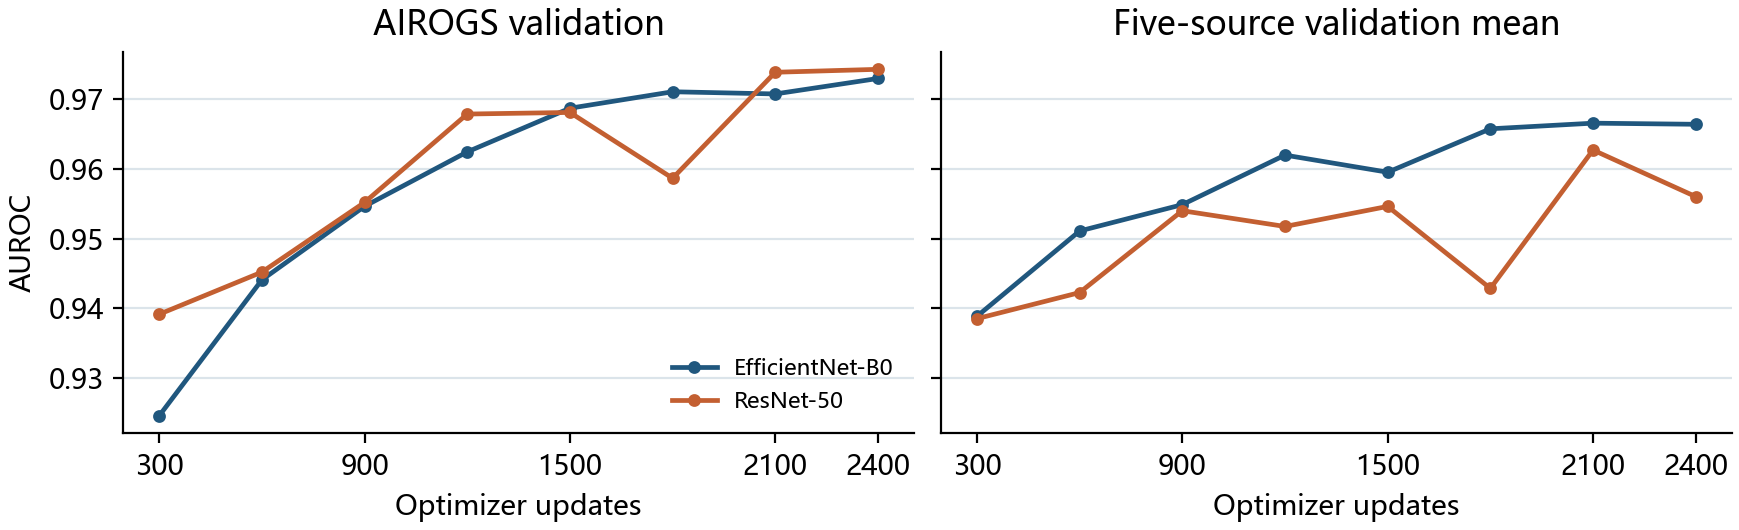
\includegraphics[width=0.96\linewidth,height=\textheight,keepaspectratio,alt={Validation AUROC every 300 updates for the two backbones. The right panel weights the five designated sources equally.}]{backbone-validation.en.png}
\caption{Validation AUROC every 300 updates for the two backbones. The
right panel weights the five designated sources equally.}
\end{figure}

The models matched on per-image draw counts, draws by source and class,
and degradation exposure. Each run made 38,384 image draws, including
repeats. Synthetic degradation was applied on 19,224 draws. ResNet-50
took about 21.5 minutes and skipped 0 updates under mixed precision.
Their AIROGS validation AUROC values at update 2,400 were 0.9729 and
0.9743, respectively.

\subsection{Next validation
priorities}\label{next-validation-priorities}

Repeat the matched comparison using the other two established seeds to
check whether the reduction in AIROGS misses recurs and extends to
pooled development. Real poor-quality originals remain scarce. The
earlier development audit found 12 human-graded poor-quality positives
and zero such negatives. Before independent testing, specify the primary
cohort, freeze thresholds and review rules, and define routing for
positive calls and disposition after a same-eye retake. The reserved
test cohorts remain sealed.

\href{backbone-results.json}{Results and input hashes} ·
\href{../../../configs/backbone_20261118/resnet50.json}{Training
configuration} ·
\href{../../../tools/analyze_matched_backbones_20261118.py}{Analysis
script} · \href{gray-zone.en.md}{Gray-zone evaluation}

\end{document}
